\documentclass[tikz,border=2pt]{standalone}
\usepackage{amsmath,amssymb}
\usepackage{pgfplots}
\pgfplotsset{compat=1.18}
\usetikzlibrary{arrows.meta}

\begin{document}
% Central moments measure the distribution around its mean: for the pmf 0.5, 0.3, 0.2 on
% 1, 2, 3 (mean 1.7) the deviations are -0.7, 0.3, 1.3; the second central moment is the
% variance and the third one records the asymmetry.
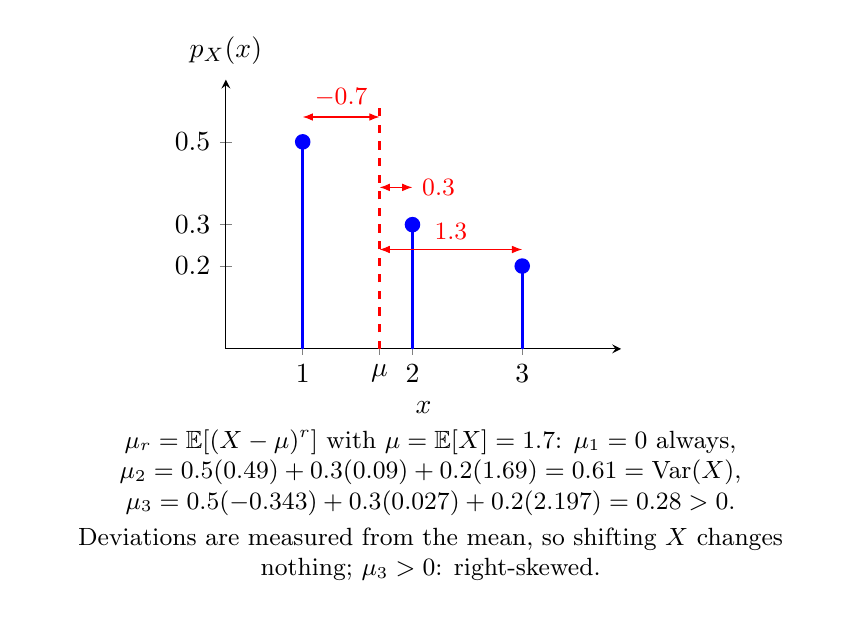
\begin{tikzpicture}
	\begin{axis}[
		axis lines=left, xmin=0.3, xmax=3.9, ymin=0, ymax=0.65,
		xtick={1,1.7,2,3}, xticklabels={$1$,$\mu$,$2$,$3$}, ytick={0.2,0.3,0.5},
		xlabel={$x$}, ylabel={$p_X(x)$}, ylabel style={rotate=-90, anchor=south, at={(axis description cs:0,1.02)}},
		width=6.6cm, height=5cm, clip=false
		]
		\addplot[ycomb, blue, very thick, mark=*, mark size=2.2pt] coordinates {(1,0.5) (2,0.3) (3,0.2)};
		\draw[red, dashed, thick] (axis cs:1.7,0) -- (axis cs:1.7,0.6);
		\draw[red, {Latex[length=1.3mm]}-{Latex[length=1.3mm]}] (axis cs:1,0.56) -- (axis cs:1.7,0.56) node[midway, above, font=\small] {$-0.7$};
		\draw[red, {Latex[length=1.3mm]}-{Latex[length=1.3mm]}] (axis cs:1.7,0.39) -- (axis cs:2,0.39) node[right, font=\small] {$0.3$};
		\draw[red, {Latex[length=1.3mm]}-{Latex[length=1.3mm]}] (axis cs:1.7,0.24) -- (axis cs:3,0.24) node[midway, above, font=\small] {$1.3$};
	\end{axis}
	\node[anchor=north, align=flush center, text width=10cm, font=\small] at (2.6,-0.9) {$\mu_r=\mathbb{E}[(X-\mu)^r]$ with $\mu=\mathbb{E}[X]=1.7$: $\mu_1=0$ always,\\ $\mu_2=0.5(0.49)+0.3(0.09)+0.2(1.69)=0.61=\operatorname{Var}(X)$,\\ $\mu_3=0.5(-0.343)+0.3(0.027)+0.2(2.197)=0.28>0$.\\[2pt] Deviations are measured from the mean, so shifting $X$ changes nothing; $\mu_3>0$: right-skewed.};
\end{tikzpicture}
\end{document}
